\section{The internals of the compiler}

A compiler is divided into several different phases: First of all, there is the source program file which is the input to the compiler. The code is scanned by the aptly named scanner phase, converting the code into a stream of tokens. The tokens of the language are the smallest units that represent something meaningful. These are then grammatically analysed, or parsed, forming what is called an Abstract Syntax Tree (AST). A semantic analysis on the AST is performed, with the help of a symbol table, which is a table of all defined identifiers and the relevant information attached to them, such as declaration, type, scope and so on. Finally the target code is generated in the target language and ready for execution. The process will be elaborated to provide a little background knowledge of the compiler construction, as described in \cite{Fischer2010}.

Below is an illustration:

\begin{figure}[ht]
	\centering
		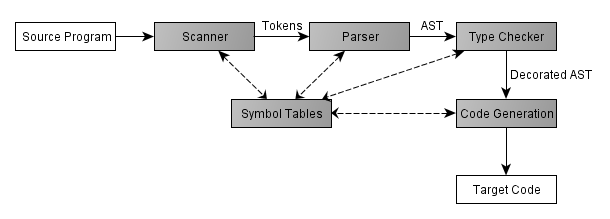
\includegraphics[scale = 0.5]{img/compiler.png}
	\caption{Compiler}
	\label{fig:compiler}
\end{figure}


\subsection{The Scanner}

The scanner is the part of the compiler responsible for transforming characters from the source program into a stream of tokens, i.e. the elementary symbols that define the language syntax, and the symbols that the parser can work with.
It is very important to have a formal definition of the tokens so that lexical rules are clearly stated and followed.
Tokens have two components: a type and a semantic value, the first indicating the token's membership in the terminal alphabet, the latter providing information about the token, if any is needed.
An example where the semantic value may not be needed is a terminal like "plus" in a simple calculator language. That terminal can only correspond to one token, namely the +. However for, say, a number it is important to have a semantic value to denote what number it is.
When the scanner tries to determine what kind of token is being scanned it will have a method that looks ahead, without removing the characters from the stream. Several algorithms for determining membership in the terminal alphabet can be employed, and often the scanner will also be instructed to skip certain parts of the code, like blanks and comment sections.
An example of the scanners token generation is shown below, with the line
\begin{lstlisting}
i a = 5
\end{lstlisting}

This generates 4 tokens: 
\begin{itemize}
\item A token of type "intdcl" (short for int declaration) with no need for a semantic value, as only the letter "i" corresponds to the type 
\item A token of type "id" with semantic value "a" 
\item A token of type "assign" with no need for a semantic value, as an assignment only corresponds to the "="
\item A token of type "inum" (short for integer numeral) with semantic value "5"
\end{itemize}

These tokens are then streamed to the parser. The process is illustrated below:
\begin{figure}[ht]
	\centering
		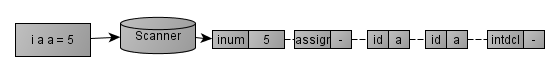
\includegraphics[scale = 0.5]{img/scanner.png}
	\caption{Scanner Phase}
	\label{fig:scanner}
\end{figure}


\subsection{The Abstract Syntax Tree}
The AST is a data structure generated by the Parser. It represents the structure of the source code. The root of the AST is the token representing the start variable in the grammar, e.g. "Program". The children of the root, and their children, are the variables or terminals that can be substituted for the parent. As an example, "Program" can be substituted with either "Decls" (declarations) or "Stmts" (statements) so these are the legal children of the root. 

\subsection{The Parser}

The parser is the phase of the compiler that generates the AST. It checks whether the tokens generated by the scanner conform to the syntactical structure defined by the grammar of the language. 

There are several ways to handle the parser problem, i.e. the problem of creating the parse tree from the token stream. Some parsers create the tree from the root to the leaves, called top-down or LL parsing, others create the tree from the leaves up, called bottom-up or LR parsing. 

Top-down parsing works by creating a procedure for each non-terminal. If, for example, there is a rule "Program $\rightarrow$ Dcls | Stmts \$" the parser determines if this is a case of a declaration or a statement by looking ahead at tokens until it knows which one it is. The term LL stands for Left to right, Leftmost derivation, which signifies that the parser reads the stream from left to right and makes leftmost derivations.

An LL(k)-parser works by looking ahead at the next k tokens to decide which production to use. Generally as low a value of k as possible is preferable as the look-ahead takes time. 

Bottom-up works by reading the stream until it has a set of tokens that fits a rule in the grammar. The LR stands for Left to right, Rightmost derivations, i.e. the parser reads the stream from left to right and makes rightmost derivations.

An LR(k)-parser reads tokens until only one production rule applies. For each node in the AST it then checks if the node and its children can generate a parent node.

The top-down approach to parsing is easy and quickly implemented and therefore often used, however they cannot parse grammars where tokens share common prefixes, or grammars with left-recursive rules, and thus LR-parsers are considered stronger parsers.

\subsection{The Symbol Table}

The symbol table is a central table accessible from all compiler phases which, as mentioned, contains all identifiers and the information that is associated with these. When the declaration of an identifier is recognised by the type checker, it is stored in the symbol table along with its scope, type, so that the next time it is used it can be retrieved from the table.

\subsection{Type Checking}
The semantic analysis creates what is called a decorated AST. It checks what is called the static semantics of each node. This means that it checks that each node is meaningful and legal with regards to type etc. for the source language. If it is, the node is decorated with type information, e.g. an assignment node can be decorated with the information that it is an assignment of an integer. Should an error be discovered, for example assignment of a string to an integer, an error message is sent out. 

A type can be defined as "any property of a program that we can establish without executing the program" \cite{Krishnamurthi2007}. The definition of types varies from language to language, but common for all is the notion that types are a certain set of values, and some operations on these values, that behave the same every time the program is run. As an example a Boolean type has only the values true and false. 

\subsection{The Code Generator}
This is where the target code is generated from the decorated AST. This phase requires detailed knowledge of the target machine, e.g. register allocation, code scheduling and so on. This phase is often coded by hand instead of using a tool, and a good code generator requires many special cases to be considered.
